\documentclass{article}

\pdfoutput=1

\usepackage{amsmath}
\usepackage{amsfonts}
\usepackage{mathtools}
\usepackage{algorithm}
\usepackage{algorithmicx}
\usepackage{algpseudocodex}
\usepackage{graphicx}
\usepackage[margin=1in]{geometry}

\graphicspath{{figures/}}

\title{A Tool for Visualizing and Analyzing High-Dimensional Clustering Performance}
\author{Justin Lin\footnote{Department of Mathematics, Indiana University} and Julia Fukuyama\footnote{Department of Statistics, Indiana University}}
\date{}

\begin{document}
\maketitle

\abstract{Technological advances have spurred an increase in data complexity and dimensionality. We are now in an era in which data sets containing thousands of features are commonplace. To digest and analyze such high-dimensional data, dimension reduction techniques have been developed and advanced along with computational power. Of these techniques, nonlinear methods are most commonly employed when working with high-dimensional data because of their ability to construct visual two-dimensional embeddings of high-dimensional data. These methods unevenly stretch and shrink space in a way that represents the data's structure in a fewer number of dimensions. However, attempting to capture high-dimensional structures in a significantly lower number of dimensions requires drastic manipulation of space. As such, nonlinear dimension reduction methods are known to occasionally capture false structures, especially in noisy settings. In efforts to deal with this phenomenon, we developed an interactive tool that enables analysts to better understand and diagnose their dimension reduction results. It uses various analytical plots to provide a multi-faceted perspective on captured structures in the data to determine if they're faithful to the original data or remnants of the dimension reduction process. The tool is available in an R package named \textit{insert name here}.}

\section{Introduction}
The potency of nonlinear dimension reduction methods lies in their flexibility, allowing them to model complex data structures. That same flexibility, however, makes them difficult to use and interpret. Each method requires a slew of hyperparameters that need to be calibrated, and even when adequately calibrated, these methods require a trained eye to interpret. For example, the two most popular nonlinear dimension reduction methods, t-SNE and UMAP, are known to generate unintuitive results (\cite{understanding UMAP}, \cite{Distill}). The results often cluster, even when no clusters exist in the data. Moreover, cluster sizes and inter-cluster distances can be unreliable. We've developed an interactive tool that analysts may use to conduct a post-hoc analysis of their high-dimensional clustering. The tool uses the minimum spanning tree (MST) to model the global structure of clusters and to provide an additional perspective on inter-cluster relationships. This allows analysts to extract more information from their dimension reduction results by making it easier to differentiate the signal and the noise.

\section{Methods}

\subsection{The Minimum Spanning Tree}
Graphs have been applied to many multivariate statistical problems. The authors of \cite{MAP test} introduced the minimal ascending path spanning tree as a way to test for multimodality. The Friedman-Rafsky test \cite{Friedman-Rafsky test}, along with its modern variations \cite{Friedman-Rafsky variation 1, Friedman-Rafsky variation 2, Friedman-Rafsky variation 3}, use the MST to construct a multivariate two-sample test. Single-linkage clustering \cite{single-linkage and MST} and runt pruning \cite{runt pruning} are both intimately related with the MST. In the context of dimension reduction, IsoMap \cite{IsoMap} makes use of neighborhood graphs, \cite{MIST example} introduces the maximum information spanning tree, and \cite{MST example} uses the MST. These methods, which fall under the category of manifold learning, use graphs to model high-dimensional data assumed to be drawn uniformly from a non-linear manifold. An accurate low-dimensional embedding can then be constructed from these graphs. It's apparent that graphs are useful for modeling high-dimensional data, especially when it comes to dimension reduction and cluster analysis. Our tool uses the MST to analyze the reliability of visualizations produced by nonlinear dimension reduction methods.

To construct the minimum spanning tree (MST), start with a set of vertices, one for each point in the data set. When an edge is added between two vertices, it's assigned a weight equal to the dissimilarity between the corresponding points. The edges of the MST are selected from all possible edges so that the sum of edge weights is minimized and there exists a path between any two vertices. We've opted for the MST for a couple of key properties. Firstly, the MST and shortest paths along it are quick to compute. Secondly, the MST contains a unique path between any two vertices, providing a well-defined metric on the data. Lastly, it provides a good summary of the data's structure. It contains as a subgraph the nearest-neighbor graph, and any edge deletion in the MST partitions the vertices into two sets for which the deleted edge is the shortest distance between them \cite{Friedman-Rafsky test}.

\subsubsection{MST Stability}
The MST is meant to provide a robust estimation of the data's global structure, and more specifically, inter-cluster relationships. As such, it should be stable in the presence of noise and unaffected by local transformations of the data. To demonstrate MST stability, we study the effect of random noise on the inter-cluster relationships explained by the MST.

To derive the inter-cluster relationships from the MST, we simplified the medoid subtree using the following procedure:

\begin{algorithm}[H]
\caption{Simplified Medoid Subtree}\label{algo1}
\begin{algorithmic}[1]
\Require MST $T = (V, E)$ with medoid vertices $m_1, \hdots, m_k \in V$
\State $T' = (V', E') \Leftarrow$ minimal subtree of $T$ containing all medoid vertices $m_i$
\State $\textrm{perplexities} \Leftarrow \{p_1, \hdots, p_m\}$
\Repeat
	\State Let $v \in V'$ with $deg(v) = 2$ and neighbors $a, b \in V'$. Let $d(v, a)$ and $d(v, b)$ be the weights of the edges connected $v$ and to $a$ and $b$.
	\State Replace $v$ and its two incident edges with an edge connecting $a$ and $b$ with weight $d(v, a)$ and $d(v, b)$.
\Until{$T'$ contains no longer contains non-medoid vertices with degree two}
\State \Output T'
\end{algorithmic}
\end{algorithm}

The simplification process essentially replaces paths of non-medoid vertices with one edge of equal length. We refer to this tree as the simplified medoid subtree and is meant to encode global inter-cluster relationships.

\subsubsection{Robinson-Foulds Metric}
To compare simplified medoid subtrees, we used the Robinson-Foulds metric \cite{RF metric}. The R-F metric was originally introduced to quantify the dissimilarity of phylogenetic trees, but the algorithm generalizes to arbitrary weighted trees. It looks at partitions of each tree created by removing individual edges, then counts the number of partitions present in one tree but not in the other. We modified the algorithm (Algorithm 2) to specifically measure the dissimilarity in medoid vertices and applied a normalization so that the distances range from zero to one.

\begin{algorithm}[H]
\caption{Robinson-Foulds Distance}\label{algo2}
\begin{algorithmic}[2]
\Require Trees $T_1 = (V_1,E_1)$ and $T_2 = (V_2, E_2)$ with medoids $m_1, \hdots, m_k \in V_1$ and $n_1, \hdots, n_k \in V_2$
\State $P_1 \Leftarrow \{\}$
\For{$e \in E_1$}
	\State $G \Leftarrow (V_1, E_1 \setminus \{e\})$ with connected components $G_1$ and $G_2$
	\State $M_1 \Leftarrow \{m_1,\hdots,m_k\} \cap V(G_1)$
	\State $M_2 \Leftarrow \{m_1,\hdots,m_k\} \cap V(G_2)$
	\State $P_1 \Leftarrow \Call{Add}{P_1, \{M_1, M_2\}}$
\EndFor
\State $P_2 \Leftarrow \{\}$
\For{$e \in E_2$}
	\State $G \Leftarrow (V_2, E_2 \setminus \{e\})$ with connected components $G_1$ and $G_2$
	\State $M_1 \Leftarrow \{n_1,\hdots,n_k\} \cap V(G_1)$
	\State $M_2 \Leftarrow \{n_1,\hdots,n_k\} \cap V(G_2)$
	\State $P_2 \Leftarrow \Call{Add}{P_2, \{M_1, M_2\}}$
\EndFor
\State \Output $\frac{\left|P_1 \Delta P_2 \right|}{2\left| P_1 \cap P_2 \right|}$
\end{algorithmic}
\end{algorithm}

\subsubsection{MST Stability Experiment}
1,500 samples were randomly chosen from the MNIST data set \cite{MNIST}. Each $784 \times 784$-pixel image was flattened into a vector of length $784^2$, so the data contain 1,500 samples in $784^2$ dimensions. A PCA pre-processing step was employed to reduce the number of dimensions to 300. The simplified medoid subtree $T$ was then calculated.

Random Gaussian noise was then added to the data and the new simplified medoid subtree $T'$ was calculated. The R-F distance $RF(T, T')$ was recorded. This process was repeated 30 times.

\renewcommand{\figurename}{Figure}
\renewcommand{\thefigure}{1}
\begin{figure*}[!b]
\centering
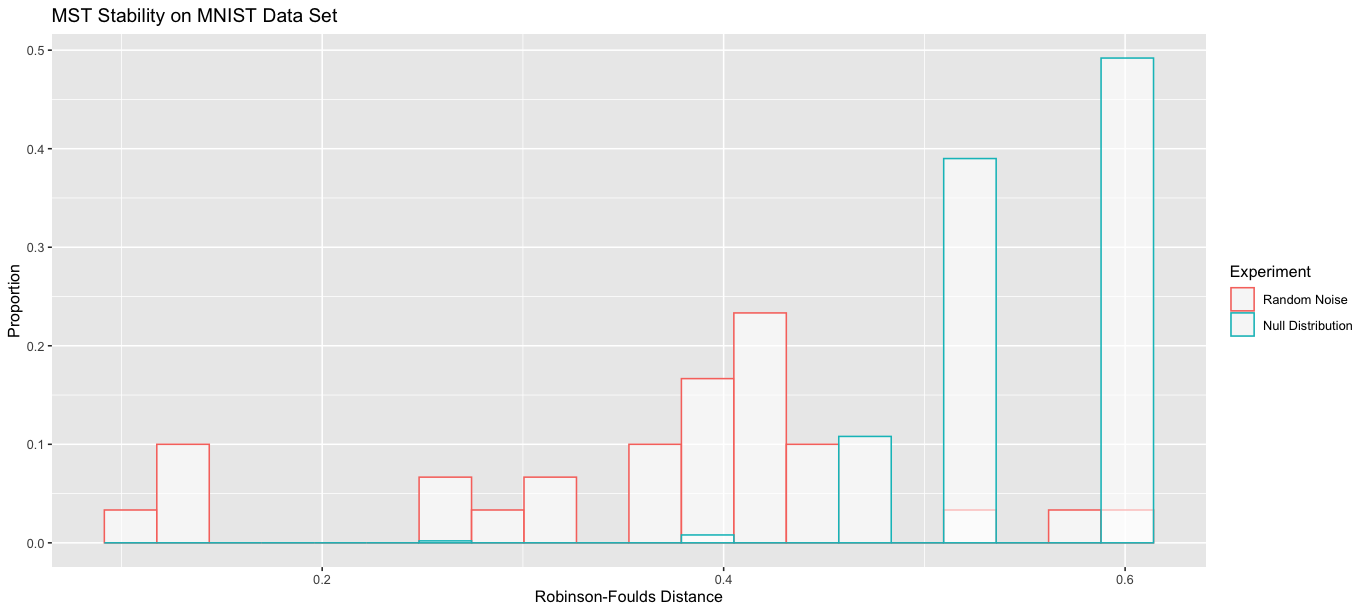
\includegraphics[scale=0.3]{RF stability}
\caption{MST Stability on MNIST Data Set}
\end{figure*}

To better interpret the R-F distances, we designed a null distribution of distances as a reference for comparison. These distances should represent R-F distances between trees that do not portray similar global structures and inter-cluster relationships. To generate the null distribution from the data, we randomly permuted the class labels and computed the R-F distances between the resulting simplified medoid subtrees and the original simplified medoid subtree. By randomly re-labelling the clusters, we are simulating examples with distinct global structures. Figure 1 shows the R-F distances produced by adding noise and permuting the class labels. The simplified medoid subtree trees generated by adding noise were significantly closer to the original simplified medoid subtree than those generated by randomly permuting the class labels in terms of R-F distance.

\subsection{The Inputs}
The interactive tool takes as input a dissimilarity matrix $D \in \mathbb{R}^{n \times n}$ representing the dissimilarities between the $n$ high-dimensional points, a two-dimensional embedding $X \in \mathbb{R}^{n \times 2}$, and a clustering $\mathcal{C} \in \{1, \hdots, k\}^n$ where $k$ is the number of classes. Optionally, it also takes a set of ID's to denote the points.

The dissimilarity matrix must be a symmetric matrix with 0's along the diagonal. The entry $D_{ij} = D_{ji}$ should represent the dissimilarity or distance between points $i$ and $j$. The chosen dissimilarity measure should be appropriate for the type of data. For example, the $L_1$ norm and even fractional $L_p$ distance measures have been suggested for high-dimensional numerical data \cite{fractional Lp norms}, Jaccard and cosine metrics are popular when working with text data \cite{text data}, and a variety of Image Distance Functions (IDFs) have been suggested for image data \cite{image metrics}. From this dissimilarity matrix, the MST is calculated.

\subsection{The Dashboard}

\renewcommand{\figurename}{Figures}
\renewcommand{\thefigure}{2a and 2b}
\begin{figure*}[!b]
\centering
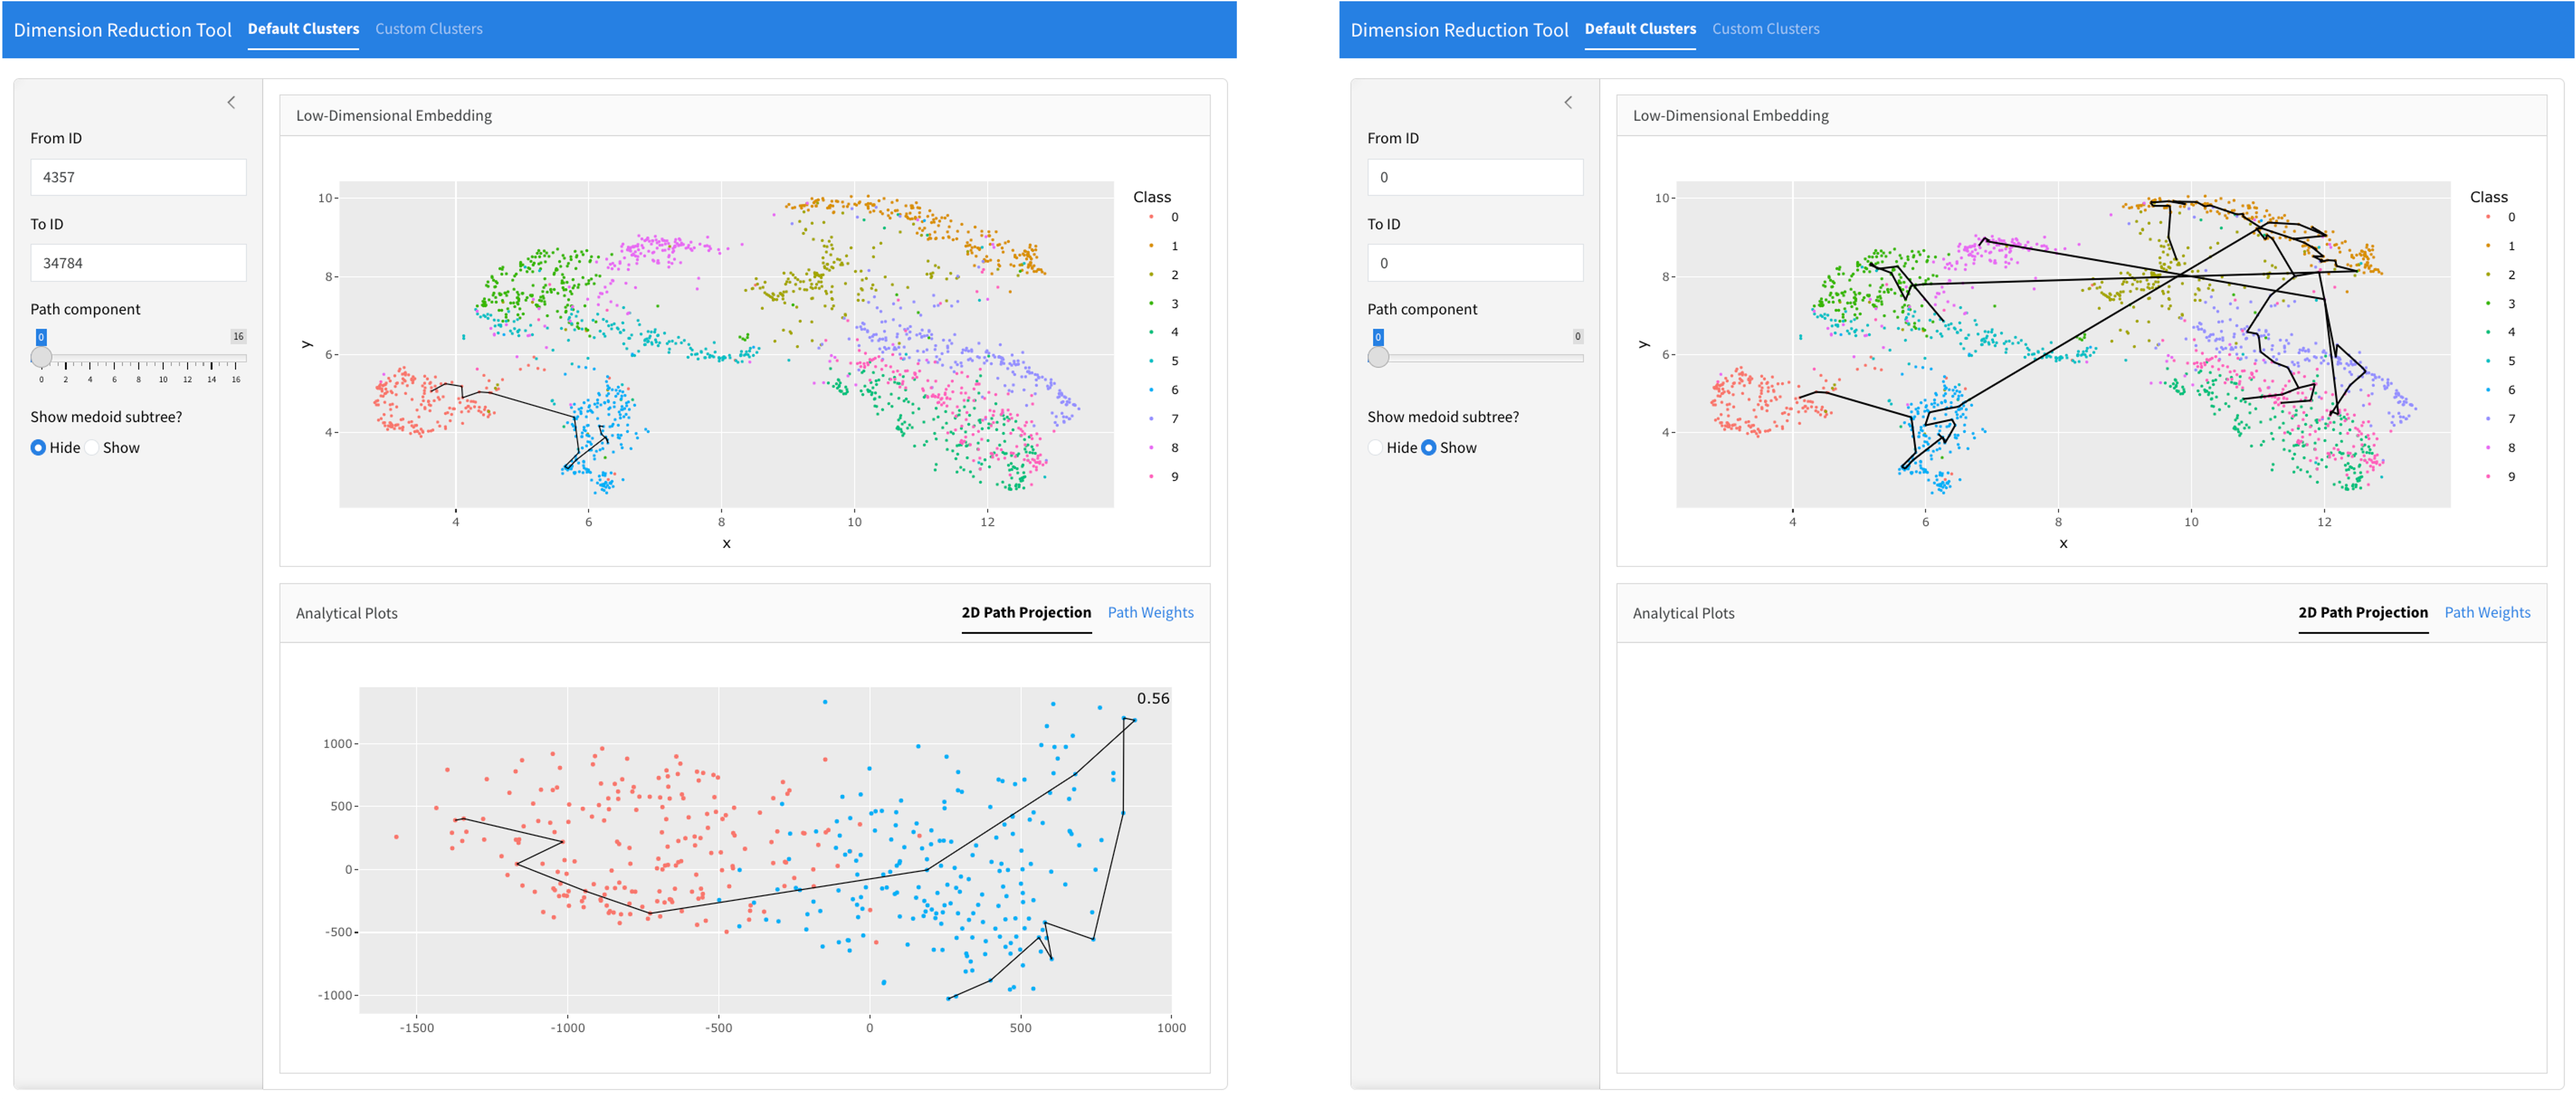
\includegraphics[scale=0.45]{dashboard}
\caption{Dashboard}
\end{figure*}

The dashboard contains two main panels as well as a side panel including adjustable settings. The first main panel depicts the low-dimensional embedding colored according to the provided clustering. The second main panel contains analytical plots. When supplied with a pair of points via ``From ID" and ``To ID", the MST path is calculated between the high-dimensional points and corresponding path in low-dimension is drawn upon the low-dimensional embedding (Figure 2a). The first analytical plot depicts a PCA projection of the high-dimensional path along with the clusters the two endpoints belong to. The PCA transform is calculated using only the points along the path then applied to the rest of the points. The number in the top right corner is the proportion of variance retained by the PCA projection. The second analytical plot contains a bar plot of path weights. The user may cycle through the segments along the path using the ``Path component" slider in the side panel. The corresponding segment will be highlighted in both the low-dimensional embedding and the 2D path projection. The corresponding path weight will also be highlighted in the plot of path weights.

To get a holistic view of the data's global structure, the user may view the medoid subtree by selecting ``Show" in the side panel (Figure 2b). The medoid subtree is the minimal subtree of the MST containing the medoid of each class. The medoid subtree describes the global arrangement of clusters.

Along the top bar, the user may also navigate to the next page named ``Custom Clusters". This page contains the same plots, but the user may instead define their own clusters of interest. To define a cluster, the user must select a subset of points by clicking and dragging along the low-dimensional embedding plot. Once the points are selected, the user can save the selected points by clicking ``Submit Group 1". The user must then repeat the process with the second cluster of points and click ``Submit Group 2". Once both clusters have been submitted, the path between the (high-dimensional) medoids of the selected clusters is portrayed. The user may also adjust the endpoints of the path. The 2D path projection will contain the points along the path together with the selected points. This page is highly useful for analyzing spacial clusters that may not be represented by the provided clustering.

\section{Results}
\subsection{MNIST}
The MNIST database is a collection of 70,000 images of handwritten digits \cite{MNIST}. Each image contains $784 \times 784$ pixels, so when vectorized, the data set contains 70,000 points in 614,656 dimensions. A random subsample of 2,000 images was taken and PCA pre-processing step was applied. The number of dimensions was reduced to 300 before applying UMAP to construct a two-dimensional visualization.

 To demonstrate how to use the tool, we analyze a hypothetical clustering instead of the true class labels. k-means was applied to the processed high-dimensional data with 10 clusters,  one for each digit. k-means does not agree with the UMAP embedding for certain clusters (Figure 3).
 
\subsubsection{Classes One and Two}
The UMAP embedding suggests classes one and two could be combined into one cluster. k-Means is known to struggle with clusters of varying sizes and densities, so it may have incorrectly separated this cluster into two classes.

To start, we navigate to the custom clusters tab and select the class one and class six points as our two groups. The path connecting the high-dimensional medoids is projected on the low-dimensional plot. The path exhibits minimal complexity and does not pass through any other clusters. Moreover, the path weights are consistent and relatively small (the path weights are scaled relative to the longest path in the MST). The edge connecting the two classes is also no longer than other edges along the path. This implies the class one and class two points are tightly packed, suggesting they represent the same digit.
 
 \renewcommand{\figurename}{Figure}
\renewcommand{\thefigure}{3}
\begin{figure*}[!t]
\centering
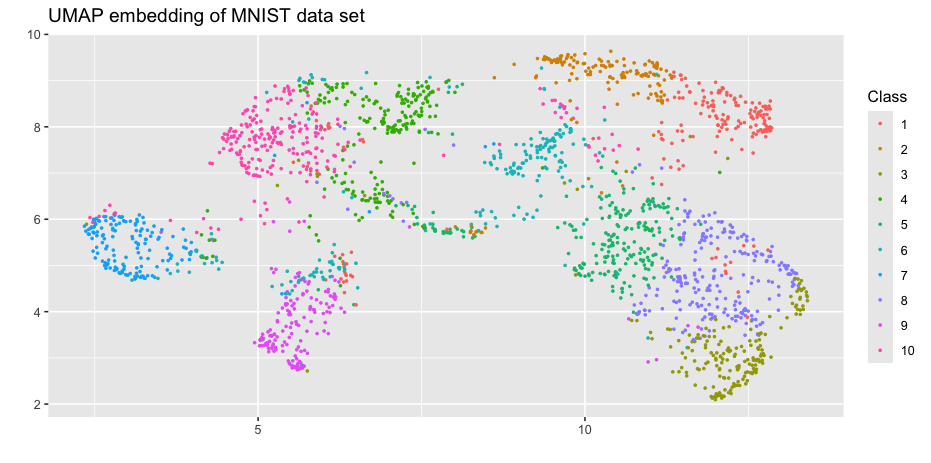
\includegraphics[scale=0.43]{MNIST kmeans}
\caption{k-Means Applied to MNIST Data}
\end{figure*}

\subsubsection{Class Four}
The class four points are split into two separate clusters. To understand their relationship, we select the clusters as our two groups then select endpoints contained in the center of each cluster. The resulting path is long and complex while also passing through various other clusters. Though the complexity is exaggerated by the low-dimensional embedding. Inspection of the path weights reveals the other clusters the path passes through are not as far away from the class four clusters as depicted. In fact, the longest segments along the path are contained within the two class four clusters. k-means is known to struggle with data with nonuniform density, so these points were grouped together due to their low density. While the circuitous path suggests the class four clusters represent separate digits, the clusters may still represent similarly looking digits.

\subsubsection{Classes Three, Five, and Eight}
Looking at classes three, five, and eight, the upper portions of each class seem to form an elongated cluster together. To determine if this is a cohesive cluster, we select half of the cluster as group one and the other half as group two. We also switch the endpoints to construct a path that spans the entirety of the cluster while also ensuring all three classes are represented in the 2D path projection plot.

The resulting path passes from class five, to class eight, then to class three. Along the way, the path also passes through a couple class one points, some within the elongated cluster and some outside. Investigation of the path weights reveals that the exterior class one points aren't nearly as far removed as depicted. The low-dimensional separation is a result of the non-linear dimension reduction. Therefore, the path connecting the endpoints of the elongated cluster is relatively direct with minimal complexity, suggesting the upper portions of classes three, five, and eight represent the same digit.

The natural follow-up is to investigate the lower portions of classes three, five, and eight. Again, we split the cluster in half to serve as our two groups and adjust the endpoints to get a path that spans the entire cluster. The resulting path passes through classes one and two as well as the cluster consisting of the upper portions of classes three, five, and eight. The path weights, as discussed previously, show the low-dimensional embedding exaggerates the distance between classes one/two and classes three/five/eight. While the path passes through other clusters, they are all nearby, so there is a lack of conclusive evidence.

\subsection{The True Class Labels}
To verify the analysis, we reference the true class labels. It was correct to combine classes one and six. Together, they represent the digit one. It was correct to separate class four into two separate clusters. The two clusters represent digits five and eight, which aligns with our hypothesis that the clusters are separate, but represent similarly looking digits. The upper portions of classes three, five, and eight do, in fact, represent the same digit. They represent the digit seven. And lastly, the lower portions of classes three, five, and eight represent the digits three and nine. These digits were tough to distinguish and very similar numerically, as illustrated by their overlapping nature in the low-dimensional embedding.

\newpage

\begin{thebibliography}{10}

\bibitem{fractional Lp norms}
Charu C. Aggarwal, Alexander Hinneburg, and Daniel A. Keim.
\newblock On the surprising behavior of distance metrics in high dimensional space.
\newblock {\em Lecture Notes in Computer Science, vol. 1973}, 2001.

\bibitem{Friedman-Rafsky variation 1}
Bhaswar B. Bhattacharya.
\newblock A general asymptotic framework for distribution-free graph-based two-sample tests.
\newblock {\em Journal of the Royal Statistical Society Series B: Statistical Methodology 81:3, 575-602}, 2019.

\bibitem{Friedman-Rafsky variation 2}
Hao Chen and Jerome H. Friedman.
\newblock A new graph-based two-sample test for multivariate and object data.
\newblock {\em Journal of the American Statistical Association 112:517, 397-409}, 2017.

\bibitem{Friedman-Rafsky variation 3}
Hao Chen, Xu Chen, and Yi Su.
\newblock A weighted edge-count two-sample test for multivariate and object data.
\newblock {\em Journal of the American Statistical Association 113:523, 1146-1155}, 2018.

\bibitem{understanding UMAP}
Andy Coenen and Adam Pearce for Google PAIR.
\newblock Understanding UMAP.
\newblock {\em https://pair-code.github.io/understanding-umap/}.

\bibitem{MNIST}
Li Deng.
\newblock The MNIST database of handwritten digit images for machine learning research.
\newblock {\em IEEE Signal Processing Magazine 29:6}, 2012.

\bibitem{image metrics}
Vito Di Ges\`u and Valery Starovoitov.
\newblock Distance-based functions for image comparison.
\newblock {\em Pattern Recognition Letters 20:2, 207-214}, 1999

\bibitem{single-linkage and MST}
J. C. Gower and G. J. S. Ross.
\newblock Minimum spanning trees and single linkage cluster analysis.
\newblock {\em Journal of the Royal Statistical Society. Series C (Applied Statistics) 18:1, 54-64}, 1969.

\bibitem{Friedman-Rafsky test}
Jerome H. Friedman and Lawrence C. Rafsky.
\newblock Multivariate generalizations of the Wald-Wolfowitz and Smirnov two-sample tests.
\newblock {\em Annals of Statistics 7:4, 697-717}, 1979.

\bibitem{MIST example}
Bracken M. King and Bruce Tidor.
\newblock MIST: Maximum information spanning trees for dimension reduction of biological data sets.
\newblock {\em Bioinformatics 25:9, 1165-1172}, 2009.

\bibitem{text data}
Abdul Wahab Qurashi, Violeta Holmes, and Anju P. Johnson.
\newblock Document processing: Methods for semantic text similarity analysis.
\newblock {\em IEEE}, 2020.

\bibitem{runt pruning}
Werner Stuetzle.
\newblock Estimating the cluster tree of a density by analyzing the minimal spanning tree of a sample.
\newblock {\em Journal of Classification 20, 25-47}, 2003.

\bibitem{IsoMap}
Joshua B. Tenenbaum, Vin de Silva, and John C. Langford.
\newblock A global geometric framework for nonlinear dimensionality reduction.
\newblock {\em Science 290:2319}, 2000.

\bibitem{MST example}
Daniel Probst and Jean-Louis Reymond.
\newblock Visualization of very large high-dimensional data sets as minimum spanning trees.
\newblock {\em Journal of Cheminformatics 12:12}, 2020.

\bibitem{MAP test}
Gregory Paul M. Roz\'al and J.A. Hartigan.
\newblock The MAP test for multimodality.
\newblock {\em Journal of Classification 11, 5-36}, 1994.

\bibitem{RF metric}
D. F. Robinson and L. R. Foulds.
\newblock Comparison of Phylogenetic Trees.
\newblock {\em Mathematical Biosciences 53, 131-147}, 1981.

\bibitem{Distill}
Martin Wattenberg, Fernanda Vi\'egas, and Ian Johnson.
\newblock How to Use t-SNE Effectively.
\newblock {\em Distill}, 2016.

\end{thebibliography}

\end{document}